\section{Einrichtung der Eclipse-Arbeitsumgebung}
Im Folgenden wird davon ausgegangen, dass die Eclipse IDE (for Java EE Developers) in der oben genannten Programmversion installiert ist.

\subsection{Installation empfohlener Eclipse Plugins}
Die Installation zusätzliche Plugins in Eclipse erfolgt über den Menüpunkt \textsc{Help / Install New Software\ldots}. In dem sich nun öffnenden Fenster kann eine \textsc{Software Site} des zu installierenden Plugins angegeben werden. Diese wird in das Feld \textsc{Work with:} eingetragen und nach einem klick auf \textsc{Add\ldots} durch Angabe eines Namens dauerhaft zu den verfügbaren \textsc{Software Sites} der aktuellen Eclipse-Installation hinzugefügt. Gleichzeitig werden alle unter dieser \textsc{Software Site} verfügbaren Plugins im unteren Bereich des Fensters aufgelistet. Durch die Auswahl der benötigten Plugins und einem Klick auf \textsc{Next} können die ausgewählten Plugins installiert werden. Die nun erscheinende Lizenzvereinbarung ist mit einem Klick auf \textsc{Ok} zu bestätigen.

\subsubsection{jBPM Plugin}
Die für eine Installation des aktuellen jBPM-Plugins (6.3.0) benötigte URL lautet: \url{http://downloads.jboss.org/jbpm/release/6.3.0.Final/updatesite/}. Für die weiteren Erläuterungen ist eine vollständige Installation aller von der oben genannten \textsc{Software Site} bereitgestellten Plugins nicht erforderlich. Zu den benötigten Plugins zählen:
\begin{itemize}\renewcommand{\labelitemi}{\itemizecheck}
	\item JBoss Drools Core
	\item JBoss Drools/jBPM Common
	\item JBoss jBPM Core
\end{itemize}
Nach kurzem laden des Inhalts, werden im mittleren Bereich die zur Installation bereitstehenden Pakete angezeigt (siehe Abbildung \ref{fig:install-jbpm-package-list}).\footnote{Farblose Icons weisen auf bereits installierte Plugins hin.}
\begin{figure}[htp]
	\centering
	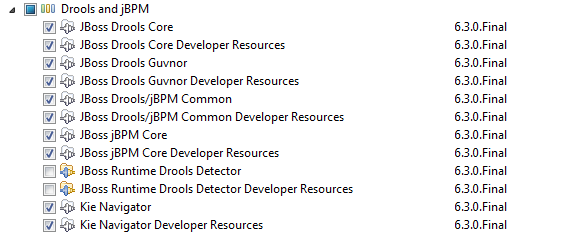
\includegraphics[width=\textwidth]{image/screenshots/install-jbpm-plugin}
	\caption{Liste an jBPM-Paketen für Eclipse-Plugin}\label{fig:install-jbpm-package-list}
\end{figure}

\subsubsection{BPMN2 Modeler Plugin}
Brauche ich davor etwas Text? Ja! Hier muss also noch etwas mehr Text stehen. Und hier steht wohl immer noch nicht genügend Text. Brauche ich davor etwas Text? Ja! Hier muss also noch etwas mehr Text stehen. Und hier steht wohl immer noch nicht genügend Text. Brauche ich davor etwas Text? Ja! Hier muss also noch etwas mehr Text stehen. Und hier steht wohl immer noch nicht genügend Text.
\begin{info}{111}
	Bei der Anfertigung dieses Dokumentes wurden folgende Programmversionen verwendet:
	\begin{itemize}
		\item \href{http://www.eclipse.org/downloads/download.php?file=/technology/epp/downloads/release/mars/1/eclipse-jee-mars-1-win32-x86_64.zip}{Eclipse 4.5.1} (Plugins: BPMN2 Modeler 1.2.1, Drools and jBPM 6.3.0)
		\item \href{http://download.oracle.com/otn-pub/java/jdk/8u66-b17/jdk-8u66-windows-x64.exe}{JavaJDK 1.8.66}
		\item \href{http://sourceforge.net/projects/jbpm/files/jBPM\%206/jbpm-6.3.0.Final/}{jBPM 6.3.0}\star
		\item \href{http://mirror.23media.de/apache/maven/maven-3/3.3.3/binaries/apache-maven-3.3.3-bin.zip}{Maven 3.3.3}
		\item \href{http://get.enterprisedb.com/postgresql/postgresql-9.4.5-1-windows-x64.exe}{PostgreSQL 9.4.5} (JDBC-Driver: 9.4-1205)
		\item \href{http://download.jboss.org/wildfly/9.0.2.Final/wildfly-9.0.2.Final.zip}{Wildfly 9.0.2}\star
	\end{itemize}
	Abweichungen von den oben genannten Programmversionen können dazu führen, dass sich die in diesem Dokument beschriebenen Beispiele (Grafiken, Quellcode-Auszüge, usw.) in ihrem Vorgehen und Inhalt unterscheiden. Für die schnelle Einrichtung wird daher empfohlen nicht von den genannten Programmversionen abzuweichen. Hierunter fallen vor allem die mit einem Stern (*) gekennzeichneten Programmversionen.
\end{info}

\xmllisting{modules.xml}{lst:xml}